% !TEX root = ../../prj4projektrapport.tex
% SKAL STÅ I TOPPEN AF ALLE FILER FOR AT MASTER-filen KOMPILERES 

\section{Design og implementering}
I dette afsnit beskrives, hvordan Måleenheden er udviklet. Måleenheden er designet til at kunne måle strøm og spænding centralt og decentralt. Spændingen måles parallelt over forbrugeren. Strømmen måles som spændingsfaldet hen over en 1$\Omega$ modstand i serie med hver forbruger og transmissionslinje. 

\subsection{Hardware}

Under udviklingen af hardwaren har det vist sig at der ikke kunne måles differentielt mellem to tilfældige punkter, men at der kun kan måles mellem et punkt og Nul. Dette gav ikke noget problem ift. målingen ved forbrugerne, men det betød at der ikke kunne måles centralt ved den viste opstilling på figur \ref{fig:MaalForanalyse}. Dette blev løst ved at flytte 1$\Omega$ modstanden ned til N, som vist på figur \ref{fig:MaalAktuel}. Der må derfor accepteres et spændingsfald over denne modstand.

\begin{figure}[H] % (alternativt [H])
	\centering
	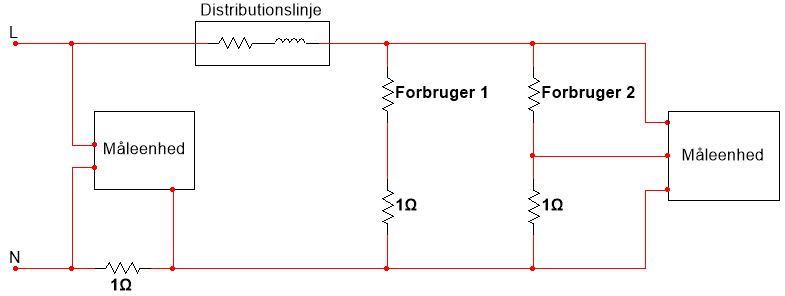
\includegraphics[width=0.8\textwidth]{figure/MaalAktuel}
	\caption{Aktuel tilslutning af Måleenhed}
	\label{fig:MaalAktuel}
\end{figure} 


\subsubsection{Hardware beskrivelse}
PSoC'ens sample område ligger mellem 0 og 5V, hvor signalerne til spændingen og strømmen forventes at svinge omkring 0V. Derfor er der udviklet hardware der kan hæve signalerne til at svinge omkring 2,5V. Måleenheden skal kunne måle op til 8V, så derfor har det været nødvendigt at dæmpe spændingssignalet. Strømniveauet er tilgengæld meget lille, hvorfor vi gerne vil forstærke det. På figurer \ref{fig:MaalHardware} ses diagrammet for hardwaren. Det er valgt at bruge operationsforstærkeren AD823, der er en rail-to-rail-forstærker, som kan forsynes med 5VDC fra PSoC'en. Yderligere information om hardwaren kan findes i dokumentationen\footnote{Projektdokumentation, 9.1, Hardware}.  
  

\begin{figure}[htbp] % (alternativt [H])
	\centering
	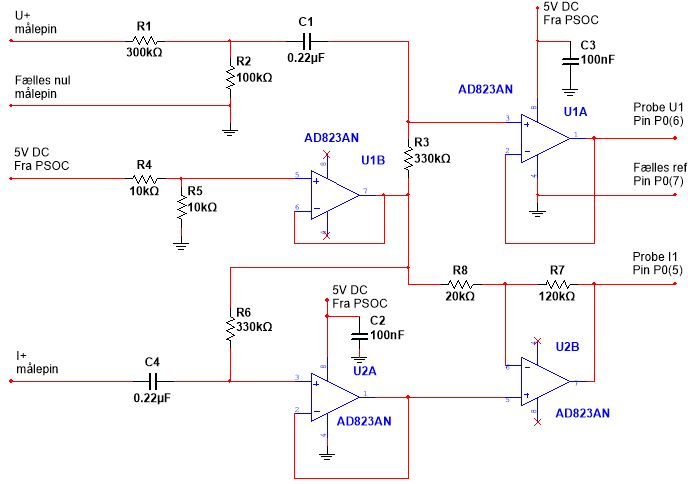
\includegraphics[width=1\textwidth]{figure/MaalHardware}
	\caption{Diagram for hardwaren til Måleenheden}
	\label{fig:MaalHardware}
\end{figure} 
 